\documentclass[msc,oneside,11pt,norunningheaders]{ubcthesiscpbl}
%[phd,10pt,noupper,runningheaders]{ubcthesis} 
\usepackage[utf8]{inputenc}  
\usepackage{setspace}
\newcommand{\ifdoDoubleSpace}[1]{}
% committee option is for draft: 1.5 spacing
%\makeatletter

\if@twoside
\def\setpageforTOC{\setcounter{page}{2}}
\else
\def\setpageforTOC{}
\fi

\if@twoside
  \def\ps@plain{%
    %\let\@oddfoot\@empty\let\@evenfoot\@empty
    \let\@oddhead\@empty\let\@evenhead\@empty
    %\def\@evenhead{%
    \def\@evenfoot{%
      \parbox{\textwidth}{%
        \makebox[\textwidth]{{\pagenumberfont\thepage}\hfill}
        %\if@headline\vspace{\headlinespace}\fi
        }%
    }%
    %\def\@oddhead{%
    \def\@oddfoot{%
      \parbox{\textwidth}{%
        \makebox[\textwidth]{\hfill{\pagenumberfont\thepage}}
        %\if@headline\vspace{\headlinespace}\fi
      }%
    }%
    }%
\fi

  \def\ps@plain{%
    %\let\@oddfoot\@empty\let\@evenfoot\@empty
    \let\@oddhead\@empty\let\@evenhead\@empty
    %\def\@evenhead{%
    \def\@evenfoot{%
      \parbox{\textwidth}{%
        \makebox[\textwidth]{{\pagenumberfont\thepage}\hfill}
        %\if@headline\vspace{\headlinespace}\fi
        }%
    }%
    %\def\@oddhead{%
    \def\@oddfoot{%
      \parbox{\textwidth}{%
        \makebox[\textwidth]{\hfill{\pagenumberfont\thepage}}
        %\if@headline\vspace{\headlinespace}\fi
      }%
    }%
    }%

\makeatother
\usepackage{phdthesis}
\usepackage{mathptmx} 
\setcounter{secnumdepth}{4}
\setcounter{tocdepth}{4}
\usepackage{varioref} % eqref is in here?????
\usepackage{url} % For a url..
\usepackage{amssymb} % amssymb/amsmath have?? checkmark? eqref?
\usepackage{amsmath} % align environment (everyone says stop using eqnarray!)


\usepackage{index}
% Following two are just black holes to accomodate index calls in the
% variable list table
\newindex{vars}{vidx}{and}{Coded variables}
\newindex{surveyvars}{sidx}{sand}{Survey variables}

\providecommand{\tabularnewline}{\\} % LyX relic

%******** natbib ********************************
% This is a very nice package for bibliographies.  It includes options
% for sorting and compressing bibliographic entries.
%\usepackage[square,authoryear]{natbib} % REMOVED OPTIONS: numbers,sort&compress,
\usepackage[square,comma,numbers,sort&compress]{natbib}

% cPbL: For chapter-level bibliographies:
%\usepackage{bibtopic}
%\bibliographystyle{aguCpbl}%cje}

%******** graphics and graphicx ******************************
% This allows you to include encapsulated postscript files.  If you
% don't have this, comment the \includegraphics{} line following the
% comment "%includegraphics" later in this file.
\usepackage{graphicx}
\usepackage{subfigure}
%******** lscape ******************************
% This allows you to include landscape layout pages by using the
% |landscape| environment. Note that this output might only be valid
% after converting to a postscript or pdf file.
\usepackage{lscape}

\usepackage{listings}


%******** psfrag ******************************
% This allows you to replace text in postscript pictures with formated
% latex text.  This allows you to use math in graph labels
% etc. Uncomment the psfrag lines following the "%psfrag" comment
% later in this file if you don't have this package.  The replacements
% will only be visible in the final postscript file: they will be
% listed in the .dvi file but not performed.
\usepackage{psfrag}

%******** afterpage ***************************
% This package allows you to issue commands at the end of the current
% page.  A good use for this is to use the command
% \afterpage{\clearpage} right after a figure.  This will cause the
% figure to be inserted on the page following the current one (or on
% the current page if it will fit) but will not break the page in the
% middle.
\usepackage{afterpage}

%%%%%%%%%%%%%%%%%%%%%%%%%%%%%%%%%%%%%%%%%%%%%%%%%%%%%%%%%%%%%%%%%%%%%%
% Allow a new preface entity which is useful for a DEDICATION
%%%%%%%%%%%%%%%%%%%%%%%%%%%%%%%%%%%%%%%%%%%%%%%%%%%%%%%%%%%%%%%%%%%%%%
% Use as follows:
%     \beforepreface
%     \dedication{To my grandparents ...}
%     \prefacesection{Abstract}   ...
%
% 2000 February 14: cPbL
\def\dedication#1{
  \chapter[Dedication]{} % Put in TOC but don't display "Dedication"
                         % on page
%  \thispagestyle{empty}  % No page number
  \thispagestyle{plain}   % Yes page number
  \vspace{6cm}
  \begin{center}
    #1
  \end{center}
  }
     
% Define a command to start a bib section for manuscript-based thesis
\newcommand{\placeSecBib}[1]{
\forThesis{
\newpage
\begin{btSect}{veblen,evolution,institutions,swb,general,urban,weather,sk} 
\chapter*{Bibliography for #1} 
\addcontentsline{toc}{section}{Bibliography for #1}
\btPrintCited 
\end{btSect} 
\end{btUnit}
}
}

\renewcommand{\listfigurename}{List of figures}
%\renewcommand{\listtablename}{List of tables}

 
% These commands are optional.  The defaults are shown.
\institution{AGH-University of Science and Technology}
\institutionaddress{Cracow, Poland}
\program{Telecommunications}

% You can issue as many of these as you have...
%\previousdegree{S.B. Physics, Massachusetts Institute of Technology, 1995}
%\previousdegree{M.Sc. Applied Physics, Stanford University, 1998}
%\previousdegree{Ph.D. Applied Physics, Stanford University, 2001}

% These commands are required.
\title{Writing scalable network applications in Python}
\subtitle{}
\author{Łukasz Marcin Dobrzański}
\copyrightyear{2009} 
\submitdate{January 2009}%\today}

\advisor{Andrzej Głowacz}
\advisortitle{Ph.D. in Telecommunications}
% One might want to override the format of the section and chapter
% numbers.  This shows you how to do it.  Note that
\renewcommand\thepart         {\Roman{part}}
\renewcommand\thechapter      {\arabic{chapter}}
\renewcommand\thesection      {\thechapter.\arabic{section}}
\renewcommand\thesubsection   {\thesection.\arabic{subsection}}
\renewcommand\thesubsubsection{\thesubsection.\arabic{subsubsection}}
\renewcommand\theparagraph    {\thesubsubsection.\arabic{paragraph}}
\renewcommand\thesubparagraph {\theparagraph.\arabic{subparagraph}}

\usepackage{relsize}
\newcommand\muchsmaller{\smaller\smaller}
\usepackage{cpblRef}
\usepackage{cpblTables}


% Below is for the data (survey appendix). Gods help me!
\usepackage{psfrag,color,graphicx}
\graphicspath{{/home/cpbl/papers/incomeCMA/plots/}{./}}

\graphicspath{{/home/cpbl/models/veblenNeighbourhoods/figuresLEL/}{/home/cpbl/models/veblenNeighbourhoods/figuresvs/}{./}{./figuresvs}{./tmpg}{/home/cpbl/papers/incomeCMA/plots/}{./}}
\usepackage{amsthm}
\usepackage{ushort} % For an underbar that looks like \bar.
\usepackage{wrapfig} % For acknowledgements only

% BELOW DEFINES THE THEOREM ENVIROS I NEED: PROPOSITION, LEMMA, PROOF
\newtheorem{theorem}{Theorem}[section]
\newtheorem{lemma}[theorem]{Lemma}
\newtheorem{proposition}[theorem]{Proposition}
\newtheorem{corollary}[theorem]{Corollary}

\newenvironment{definition}[1][Definition]{\begin{trivlist}
\item[\hskip \labelsep {\bfseries #1}]}{\end{trivlist}}
\newenvironment{example}[1][Example]{\begin{trivlist}
\item[\hskip \labelsep {\bfseries #1}]}{\end{trivlist}}
\newenvironment{remark}[1][Remark]{\begin{trivlist}
\item[\hskip \labelsep {\bfseries #1}]}{\end{trivlist}}

% Some tools to differentiate between thesis version and journal
% manuscript version.
\newcommand{\forThesis}[1]{#1}
\newcommand{\forPaper}[1]{}



\newcommand{\LELcfig}[1]{\includegraphics[width=0.75\textwidth,keepaspectratio]{#1.\epspdf}}%{\input{#1}.tex}
% Above redundant: see cpblRef.sty LELwfig

\newcommand{\epspdf}{pdf}%{eps}%
\newcommand{\cmykrgb}{cmyk}%{rgb}
\newcommand{\rawplotspath}{/home/cpbl/models/veblenNeighbourhoods/plots/raw/}
\newcommand{\iCMArawplotspath}{/home/cpbl/econ/favouritePlots/cityScatterPlots/}%{papers/incomeCMA/plots/raw/}
\usepackage[footnotesize,bf]{caption} % Does this actually call caption2 or caption3?
\setlength{\captionmargin}{20pt}


% Inconspicuous hyperref -- very nice.
  \usepackage[   
       colorlinks,
      citecolor=black,
       filecolor=black,
       linkcolor=black,
       urlcolor=black  
   ]{hyperref}

\newif\ifNBER

%%% TURN OFF COMMENTS:
\renewcommand{\draftComment}[1]{}
\renewcommand{\safeDraftComment}[1]{}
\renewcommand{\cpblOldComment}[1]{}

% Turn on comments:

%\renewcommand{\draftComment}{\draftCommentColouredBox}
%\renewcommand{\cpblOldComment}{\draftCommentColouredBox}
 
% UBC has strange format requirements, but some things not strict. So
% don't worry about things looking nice. Widen so I can fit my big tables:
% To ensure that the margin fiddling for the huge/wide/long tables
%\addtolength\oddsidemargin{-1cm}
%\addtolength\evensidemargin{-1cm}
%\addtolength\textwidth{2cm}
\addtolength\oddsidemargin{-1cm}
\addtolength\evensidemargin{-1cm}
\addtolength\textwidth{2cm}
\addtolength\textheight{3.4cm}


\newcommand{\starsOrColours}[2]{#1}

\ifdoDoubleSpace{\doublespacing}
\begin{document}
%\renewcommand\baselinestretch{1.0}

\ifdoDoubleSpace{ \begin{singlespace} }

% This starts numbering in Roman numerals as required for the thesis
% style.
\frontmatter

% The order of the following components is preserved.  The order
% listed here is the order currently required by the library.
\maketitle
\newpage\thispagestyle{empty}\newpage  %\pagestyle{empty}

\begin{abstract}
\setcounter{page}{2}

My application named SmartNotes is mend as a tool helping to keep our notes always actual and ready to use. Disregarding whether we fly by plane, work in the office, use different machines with different operating systems, or just only occasionally are connect to Internet our notes will stay synchronized in all the places we may want to always with the latest available version. Its key features are availability and scalability that combine the power of Google infrastructure with Mercurial a popular Version Control System.

\end{abstract}


\newpage\thispagestyle{empty}\newpage  %\pagestyle{empty}
\setpageforTOC

\tableofcontents
%\listoftables
\listoffigures

\chapter{Acknowledgements}
This is to thank those for whose support and criticism I could constantly count on
while working on my thesis. I will list them in alphabetical order:

\begin{itemize}
\item My parents thanks who I had the chance to study and who always believed in me.  
\item Dh.D. Andrzej Głowacz for his advices. 
\item Anna Pawłowicz thanks who I had the best motivation ever and I could always count on.
\end{itemize}

Thank You all very much!

\emph{Special mention:} Thanks to the people whose work I used while working on my project.
Thanks to all for who Open Source became a pattern for developing software.


%\dedication{\Large \em
%For Iris: this one --- and I promise it's the last --- is for you,\\
%who set me on this hidden path in 2000,\\ \vspace{5mm}
%And in memory of Robert, who had so much left to say.
%}
		
\newpage				% Force a new page.
\thispagestyle{plain}		% Suppress the running headers for this page only.
\mainmatter			%Now regular page numbering begins.

\ifdoDoubleSpace{ \end{singlespace} }

\chapter{Introduction}
\label{sec:Introduction}
Creating network applications nowadays might be a complicated process of design which involves long series of research and experiments or, on the other hand, it might be a fairly simple procedure that takes only a tenth of its time and effort. In both cases, the most frequent evaluation metric is the scalability of the application, more than a thousand of lines of code or the complexity of the model. With the rise in popularity, the usage of network applications increases, which in consequence results in an increase in the frequency that the application is requested to serve its functionality. This growth can be calculated and included at the planning level, thus becoming a good programming practice that places itself close to other widely approved design patterns. With no doubt is scalability starting to play a more important role, being often set at the same level with such issues like portability or security[quote]. The present thesis aims to introduce an application that by its original functionality would heave the potential to become a heavy traffic network application with numerous active users. In this chapter the reader can find an overview of popular notes taking applications, understand the basis of Version Control Systems, and learn about more technical sections regarding the Python programming language as well as terms of scalability in a Google App Engine product. % Introduction,Theory
\chapter{System Concept}\label{chap:concept}
The following chapter will cover the system concept, the functionality it offers and the general functional system description. Also, the following sections should clarify how the SmartNotes application can be used, illustrate its design using the UML diagrams and prepare the reader for more detailed system description included in the chapter~\ref{chap:sys_description}.

The idea of SmartNotes has been inspired by the Google Notebook application which was being actively developed until January 2009, when Google announced that further development work on this project is stopped. Google Notebook has an interesting interface and features, some of them already motioned in section~\ref{subsec:google_notebook}. what was still missing from the functionality until January 2009 was comfortable notes usage without network connectivity. The aim of the subject of the thesis was to use the idea of making a truly scalable notes taking application that would be even more flexible.

\section{Functionality description}\label{sec:functionality_descr} 
Detailed description of how a system may be used should by of utmost importance both to the developer and to the end user, as it helps gain a general perspective, called 10,000-foot view\cite[page 49]{uml_use_case}, of the system and make useful observations. The implementation as well as the conceptual and system design decisions become a side issue, as the foreground is always occupied by the functionality  the application is to offer. For that reason, the use of case scenarios and flow charts will be very helpful in describing the efficient way of using the SmartNotes application.

Users willing to work on their notes disregarding network connectivity will need to install iSmartNotes, which is a graphical interface of SmartNotes. Specifically, the SmartNotes application is divided into the web-based system and the graphical desktop interface, a separation with which UI experiments can be done without the need of having the web browser open in order to work on the notes. The web based part of SmartNotes makes the synchronization feature possible and allows to monitor the entire system of SmartNotes. However, in order to use the synchronization feature, the iSmartNotes needs to be activated by the user. Additionally, since users of SmartNotes are expected to have a Google account\footnote{Creating a Google account by visiting \url{https://www.google.com/accounts/} gives a access to various services offered by the Google company where Gmail, Google News or Google Finance are one of the most popular tools. These are regarded secure and solid services users can relay on.} the activation code will be available after logging in to the SmartNotes system with that account. This process is illustrated on figure~\ref{fig:ismartnotes_activation}. The idea behind it is to make the use of the popular Google Account and not multiply the accounts to services that the user has to know the login and password. Basing on the activation key, the user is granted access to his personalized SmartNotes account and to the synchronization feature. Without the activation, iSmartNotes can be used as a regular notes editor.  
\begin{figure}[ht]
\begin{center}
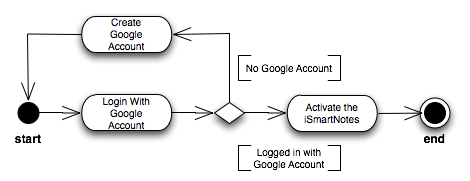
\includegraphics[scale=0.65]{charts/activate_iSmartNotes.png}
\caption{The iSmartNotes application activation with the Google Account.}
\label{fig:ismartnotes_activation}
\end{center}
\end{figure}
The skim of functionality offered by iSmartNotes is demonstrated on figure~\ref{fig:workon_ismartnotes}.
\begin{figure}[ht]
\begin{center}
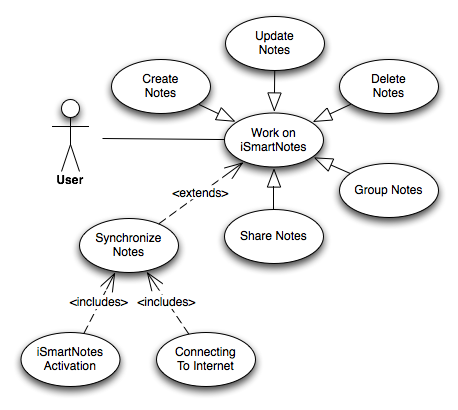
\includegraphics[scale=0.55]{charts/work_on_iSmartNotes.png}
\caption{The iSmartNotes application use cases.}
\label{fig:workon_ismartnotes}
\end{center}
\end{figure}
This includes the CRUD operations and three extra features. Firstly, the notes can be easily grouped together in named tabs, which should make organizing and finding notes much easier. Secondly, it is possible to publish the notes marked as shared. The final feature is the synchronization process that requires iSmartNotes activation and network connection to contact with the web-based part of SmartNotes. What remains to be discussed is the cooperation between iSmartNotes and the web-based part of SmartNotes, therefore, the relation between them and the functionality offered to the user and administrator are shown on figure~\ref{fig:ismartnotes_smartnotes}. 
\begin{figure}[ht]
\begin{center}
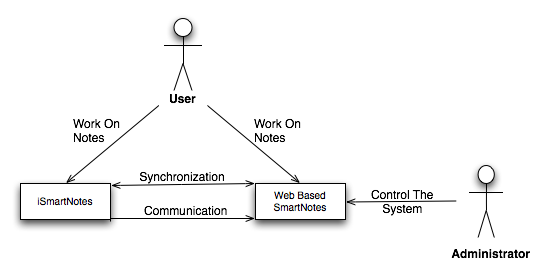
\includegraphics[scale=0.55]{charts/iSmartNotes_SmartNotes.png}
\caption{The cooperation of iSmartNotes and web based SmartNotes.}
\label{fig:ismartnotes_smartnotes}
\end{center}
\end{figure}

This interesting concept allows the user to work on iSmartNotes as well as the Web-based part of SmartNotes exchangeably, at the same time letting the SmartNotes application care for work synchronization, which has been also highlighted in the above discussed picture. Yet, however functional and elastic the application may seem, the same functionality is not feasible in the web interface of the present project, even if the administrator is granted access to tools like datastore data browser, system status or application dashboard described in section~\ref{sec:gae_general}. This can help to quickly diagnose faults within the application and rollback it to the latest stable version. Moreover,  it can indicate that the rescuers are not sufficient to serve the traffic and eventually extend them. The tools work effectively in cooperation with Google Webmaster Tools and the Google Analytics as they can provide more information concerning the web page and its visitors.

It appears to be worth describing the synchronization feature in more detail. The feature is realized by the VCS which was introduced in section~\ref{sec:popular_vcs}. No matter if the user works online or not, they have full access to notes and synchronize them online. As it has been marked on the graph from figure~\ref{fig:ismartnotes_smartnotes}, the synchronization process is bidirectional: it is triggered from the web-based part of SmartNotes, which plays a role of the main server, and the iSmartNotes, playnig the role of clients and reverse. This type of set-up should allow to update the notes whenever necessary. Another point presented in figure~\ref{fig:ismartnotes_smartnotes} is the directional communication between iSmartNotes and SmartNotes, which should be understand as an additional logic allowing to perform operations on the user side by the help of iSmartNotes, including the display of user information on significant events like availability of new features or versions.  As a matter of fact, the process is directional in one way as it is the iSmartNotes application which receives the information from the SmartNotes server and displays it to the user. Whereas the presented functionality does not fully exploit the possible feature list, as mentioned in section~\ref{subsec:vcs_comparison}, it is a good practice to keep the application as simple as possible and focus on a set of clearly defined key features.

\section{Functional description}\label{sec:functional_descr}
The SmartNotes application should run on a infrastructure that can ensure complete availability and high load. Easy system maintenance and openness to future expansion in functionality are also strongly desirable features. It is not pointless to mention that the above requires resource usage, which makes the financial model of utmost importance and is the already introduced 10,000-foot view of system requirements. Adding a friendly deployment methodology and good documentation is what would satisfy the most demanding developer.

Admittedly, in order for the application to gain popularity, users should be well informed about the application and its functionality; also, it is vital to provide availability of instructions on how to get started. For these reasons, the landing page should be not only informal and practical, but also international to reach greater group of users.

From the architectural point of view, SmartNotes is a simple client-server application, the only difference being the usage of DVCS, which allows the machines to access thesame set of commands and make their hard disks hold the entire repository with its history. Yet, it may be confusing that it still remains a client-server architecture, but just as the centralized VCS do not recognize any other architecture than the client server, the distributed VCS uses it as one of possible use cases. In the following scenario one of the machines fulfills a role of the reverential server to which all remaining machines direct their requests, at the same time being a for of public repository with the most recent version that should be always available to users. In consequence, each client requires the installation of DVCS as one of the main components, while the size of the chosen VCS matters as much as its performance, which all in all has significant impact on the final performance of iSmartNotes. For optimum user experience, the iSmartNotes application provides an easy-to-install package that could be downloaded from the server serving static content, which is not only a faster solution from dynamically served content, but also allows to save system resources, costing a minimum of CPU time.

The next two sections state certain problems related to synchronization scenarios using VCS and the application activation. They will be analyzed focusing on the evaluating of a number of possible solutions and the argumentation will lead to the choice of the most optimal solution.  
 
\subsection{Synchronization scenarios using version control systems}\label{subsec:sync_scenarios}
It is one of the main responsibilities of version control systems to keep the repositories updated. Nevertheless they never perform update without a user request\footnote{This means that the user has to run an appropriate command or click on the right button when using a graphical interface. It could be naturally automated by writing a script that would perform that task for the user or by setting a cron job with a desired time interval, but the tool still requires the user to trigger the update process.}, the reasons for which are various, but dealing with conflict situations like the one shown on figure~\ref{fig:google_notebook} seams to be the most important. To put it in simple words conflict situation it is a situation when the VCS needs the user decision to resolve the conflict situation as it cant decide which from the concurring versions should be chosen. The way the merging is done differs with different version control systems but from the user perspective operations such like update and merge are quite easy to imagine. 

Due to lack of clarity in terminology including this basic operations of version control some additional explanations needs to be done. Mercurial implements \texttt{fetch} command  which includes three steps in the listed in  the order of execution:
\begin{enumerate}
\item{Lookup.}
\item{Getting changesets\footnote{Thist is a term used mainly in Mercurial related documentation to refer the data structures used for storing the differences between revisions. This seam to be more accurate then saying 'changes' or 'differences' and will be used in this document when concerning data structures.}.}
\item{Updating or merging.}
\end{enumerate}
The first two Mercurial implements as \texttt{pull} command and the last one has two commands called respectively \texttt{update} and \texttt{merge}. On the other side in the git system \texttt{fetch} does the same that Mercurial \texttt{pull} command and the git \texttt{pull} is a substitute for the \texttt{fetch} from Mercurial. To avoid confusion in the following document the terminology from the git system will be used.

The iSmartNotes needs to make three functional operations possible: 
\begin{itemize}
\item{Update -- getting newer versions from the main server what will be called down-side synchronization.}
\item{Apply changes -- this includes operations of creating, updating and removing content.}
\item{Synchronize -- more specifically up-side synchronization to the main server.}
\end{itemize}
All of this are essential to realize the full set of iSmartNotes use cases which were generalized under the term \textit{Work on iSmartNotes} on figure~\ref{fig:workon_ismartnotes}. The sequence diagrams~\ref{fig:seq_update},~\ref{fig:seq_commit} and~\ref{fig:seq_commit2}  demonstrate how this operations could be decomposed into some lower level calls. The operation of applying changes and synchronizing was presented in one sequence as all of the sequences make an assumption of network connectivity which allows to join them easily. Without it the operations are much more simple as they become limited to the interaction between the client repository and the client application. Terms client and server are used intentionally instead of the application specific names to stress the client-server architecture and make the examples more general.

First of the diagrams illustrates internal relation of operations needed to perform the pull operation. Additionally the order in which this operations are being executed can be observed by reading the sequence diagrams from the top to bottom.
\begin{figure}[ht]
\begin{center}
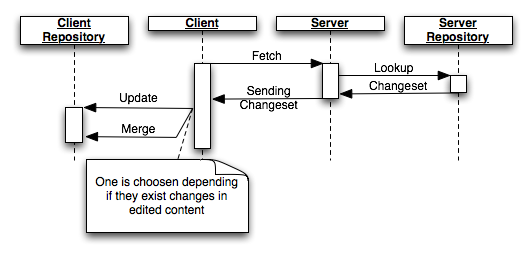
\includegraphics[scale=0.6]{charts/seq_update.png}
\caption{The pull operation sequence diagram.}
\label{fig:seq_update}
\end{center}
\end{figure}
The operation is started by the client by requesting changesets from the server and finishes after update or merge operation is performed on the client repository. As noted on figure~\ref{fig:seq_update} the condition deciding which of them should be chosen depends on existence of changes in the edited content. If merging is not needed then the update operation is done. When no chengsets are found then none of this is needed. That is a general rule when choosing between merge and update and for this reason that note wont be repeated on the following figures. It is also in common that on the sequence diagrams the client and server repository were separated from their version control repositories. By this concept front-end and back-end functions could be presented simultaneously. 

Figures~\ref{fig:seq_commit} and~\ref{fig:seq_commit2} are the product of  dissertation on what sequence of operations should be called to get a updated version after applying changes. The first one illustrates an idea of performing a \texttt{pull} first after the changes are saved in the clients repository and the \texttt{push} a the end of sequence. The opposite order is presented on figure~\ref{fig:seq_commit2} where \texttt{pull} is followed by \texttt{push}. 
\begin{figure}[ht]
\begin{center}
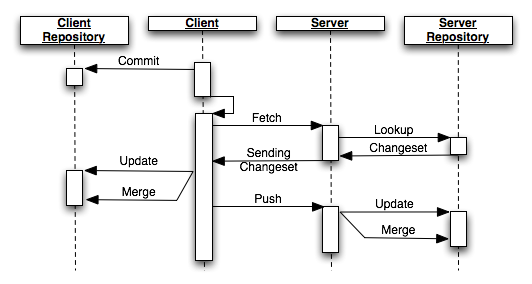
\includegraphics[scale=0.6]{charts/seq_commit.png}
\caption{The commit operation together with pull preceding the push operation.}
\label{fig:seq_commit}
\end{center}
\end{figure}
\begin{figure}[ht]
\begin{center}
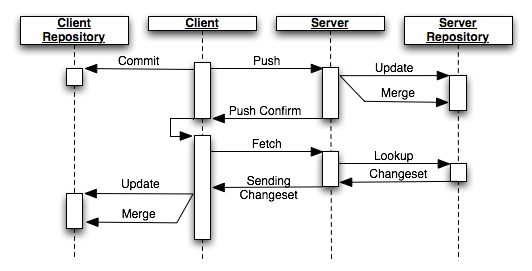
\includegraphics[scale=0.6]{charts/seq_commit2.png}
\caption{The commit operation that makes push follow the pull operation.}
\label{fig:seq_commit2}
\end{center}
\end{figure}
\newline Both of those attempts have its advantages and disadvantages. On balance the first concept appears to outperform the second one by characteristics:
\begin{itemize}
\item{The basic client action gets faster finished as it only saves the changes in the client repository.}
\item{Lower probability that the server will need to perform the merge operation. That allows to save the CPU resources and makes the application more scalable as the merges are done on the client application side. That also to solve eventual conflicts before the changesets will reach the server.}
\item{Better user experience as an effect that the changes are available in the interface offered by the client application sooner.}
\end{itemize}
From the other side the second concept ay seem more reliable as it gives grater priority to saving changesets both in the client and server repositories and preforms commit and \texttt{push} as the fist ones. That makes not that a big difference in practice and gets outweigh by the arguments mentioned above.




\subsection{iSmartNotes activation process}\label{subsec:ismartnotes_activation}
 % System concept
\chapter{System Evaluation}\label{chap:eval}
\section{Final result presentation}\label{sec:result} 
\section{Performance tests}\label{sec:performance}  % System description
\chapter{System Description}\label{chap:sys_description}
The present chapter covers the system design including specific solutions that have been chosen for the realization of the SmartNotes application. The system concept, introduced in Chapter~\ref{chap:concept}, will become extended by describing certain elements of implementation and problems found during the development process. This should allow the reader to have a deeper view into the SmartNotes application, including the functions that it offers as well as the platform that it runs on.
\section{Google App Engine platform}\label{sec:gae}
Google App Engine seems to be an outstanding development platform. For all the reasons mentioned in~\ref{sec:gae_general}, it has been decided to be used as the main platform for SmartNotes as the one preceding any other hosting services. Besides, GAE appears to be highly competitive in terms of cost calculations, which are described in Section~\ref{subsec:gae_calculations}. After registering the application with a unique name, it can be easily uploaded to Google and after a few seconds it is accessible to its users.

*****As stressed in Section~\ref{subsec:sync_scenarios}, synchronization scenarios use the client-server architecture. When running on GAE platform which is, as mentioned in~\ref{sec:gae_general}, a distributed vault-tolerant infrastructure where two subsequent request may be served by different machines located in separate data centres. Thus from the addressing scope the application can still be treated as a centralized server. In case the application requires state awareness it is the developer's role to make it so. Otherwise, the fact that the application is served from multiple machines is completely transparent from the functional point of view.

SmartNotes uses only some of the components supported by GAE and t he ones which make a part of SmartNotes application with relation with other third-party elements are presented in Figure~\ref{fig:smartnotes_components}. This is especially important as it presents all the application top level components together with marked interfaces between the particular functional blocks. This particular diagram strongly corresponds with the diagram from Figure~\ref{fig:ismartnotes_smartnotes}, which in a more general way presents the cooperation of SmartNotes and iSmartNotes with differentiated roles of the administrator and the user. 

The most complicated structure is the SmartNotes component, which is marked as an individual system. It does not require the iSmartNotes to realize its functionality. For this reason, the SmartNotes component could work with any kind of client application using the interface that the tool provides, or the interface of Mercurial HTTP chains of requests and responses that needed a back-end redesign to accommodate conditions set by GAE. The issues connected with the cooperation of Mercurial and GAE are the topic of Section~\ref{sec:hg_on_gae}. 

Furthermore, SmartNotes uses three additional interfaces which are used to interconnect the Google App Engine component with Mercurial adopted to run on GAE as well as separately, admin and user interfaces provided by SmartNotes. Each of the three components is connected in a different way. Whereas the webapp framework has a low Python overhead as mentioned in Section~\ref{subsec:webapp} and was chosen to serve the connection between the Mercurial and the Google App Engine componet, for performance reasons, it is Django which is the best choice when it comes to building nontrivial web-based functionality for reasons mentioned in Section~\ref{subsec:django}. The remaining two elements used by the GAE subsystem are the Google Account and the Datastore. The role of the first one has been presente in detail while discussing the iSmartNotes activation process in Section~\ref{subsec:ismartnotes_activation}. Some of the Datastore details will be covered in Section~\ref{sec:hg_on_gae}. 
\begin{figure}[ht]
\begin{center}
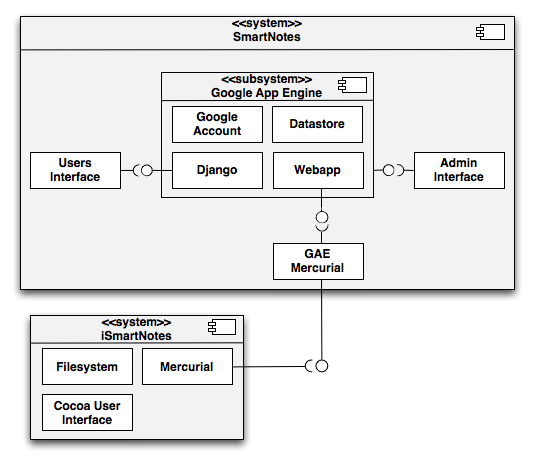
\includegraphics[scale=0.6]{charts/smartnotes_componets.png}
\caption{The components diagram of  the SmartNotes application with marked interfaces between the functional blocks.}
\label{fig:smartnotes_components}
\end{center}
\end{figure}

The second independent system is the iSmartNotes component, which remains independent until the user decides to activate it to use the synchronization feature. For this purpose, it requires a Mercurial server to interact with. The iSmartNotes, as presented in Figure~\ref{fig:smartnotes_components}, is build with three components. Firstly, the file system of the client's operating system which is the classical space where VCSs allocate their repositories. Secondly, Mercurial VCS which on the client site does not require any modifications. Finally, the Cocoa user interface whose presentation is provided in Section~\ref{sec:cocoa}.

\subsection{Financial calculations}\label{subsec:gae_calculations}
The role of this section is to introduce some basic calculations that should give the reader a general experience of what kind of resources will be used by the application with the connection to the billing rates set by Google. In the next step this values will be used to predict the order of size for monthly cost of running the application for  one million of SmartNotes users. This should should help to indicate the system elements that generate highest price of resource usage what in the end lets to concentrate on optimization in those specific area. 

Calculations bellow aim to predict theoretical monthly cost of running SmartNotes applications for one million of users with unit price detailed in Table~\ref{tab:gae_cost}. Each of resources will become briefly introduced with short explanation of taken assumptions. The outcome of this considerations is illustrated in Figure~\ref{tab:gae_cost}.
\begin{table}[h]
\centering
\caption{Google App Engine billing rates on September 2009.}
\label{tab:gae_cost}
\begin{tabular}{|l|l|l|} \hline \hline
\textbf{Resource} & \textbf{Unit} & \textbf{Unit cost} \\ \hline \hline
Outgoing Bandwidth & Gigabytes & \$0.12 \\ \hline
Incoming Bandwidth & Gigabytes & \$0.10 \\ \hline
CPU Time & CPU hours & \$0.10 \\ \hline
Stored Data & Gigabytes per Day & \$0.005 \\ \hline
Recipients Emailed & Recipients & \$0.0001\\ \hline \hline
\end{tabular}
\end{table}

Resource usage to price calculations:
\begin{itemize}
\item{\textbf{Outgoing Bandwidth}. This value represents a summarized amount of data send from the server to the users. That normally includes html, css, java script and graphic files as the standard web pages components. In classical case a total size of a web page is round \mbox{70--150KB} what with compression can reduce it by factor of about 40\%. In case of SmartNotes application the content sent between the server and iSmartNotes are the changesets. It was assumed that the size of average downstream changeset won't exceed 2KB. It is smaller from the upstream changeset as not all server responses contain a changeset. A changset is sent only if there is a need for it what happens when there application encounters differences requiring to be synchronized.   

Next made assumption regards the users activity. As stated in the beginning the calculations are done for one million of users. Additionally among this users there is a strong group of active users what translated into numbers would mean that about 80\% of users generate four editing actions. This accordingly to the synchronization scenario from Figure~\ref{fig:seq_commit} might require sending the data from and to the server.  For this reason the the bandwidth calculations for incoming and outgoing traffic use the same number of requests. This all leads to the fallowing numbers:

$Outgoing\ Bandwidth =  80\% \cdot 1,000,000\ users \cdot 4\ requests\ per\ user \cdot$\\ \hspace*{37mm} $2KB\ per\ request \cdot 30\ days \approx \textbf{183GB\ per\ month}$ \\ 
$Outgoing\ Bandwidth\ Cost = 183GB\ per\ month \cdot \$0.12\ per\ GB \approx \textbf{\$22 per\ month}$ }

\item{\textbf{Incoming Bandwidth}. In this case the same number of requests will be used just as in case of outgoing bandwidth. That is 3,200,000 of requests per day and it will be used as basic parameter in all of undermentioned calculations. 

The size of a single request will be double the value taken when calculating the outgoing bandwidth. This is cause each of the operations done by use of iSmartNotes requires sending a changeset. Remaining part of calculations regarding incoming bandwidth follows the numbers which were used for outgoing bandwidth:

$Incoming\ Bandwidth =  3,200,000\ requests\ per\ day \cdot 4KB\ per\ request \cdot 30\ days$\\ \hspace*{33mm} $\approx \textbf{366GB\ per\ month}$ \\ 
$Incoming\ Bandwidth\ Cost = 366GB\ per\ month \cdot \$0.1\ per\ GB \approx \textbf{\$37 per\ month}$ }

\item{\textbf{CPU Time}. This calculation was done by checking the average time that the CPU was idle during serving a single request. As mentioned in Section~\ref{subsec:webapp} has lower Python overhead and for performance reasons it was chosen over the Django framework. This in consequence allowed to reduce the CPU time parameter. Due to the fact that all requests require CPU time the base number of 3,200,000 requests per day is multiplied by two for upstream and downstream requests. Turning that into numbers gives:

$CPU\ Time =  3,200,000\ requests\ per\ day \cdot 2 \cdot 0.02\ seconds\ per\ request \cdot 30\ days$\\ \hspace*{17mm} $\approx \textbf{1067\ hours\ per\ month}$ \\ 
$CPU\ Time\ Cost = 1067\ hours\ per\ month \cdot \$0.1\ per\ hour \approx \textbf{\$107 per\ month}$}

\item{\textbf{Stored Data}. To help imagine the storage space needed for an average notes repository let say that the popular collection of stories called "Winnie-the-Pooh" contains about 4,000 lines and it size in plain text without graphics is about 150KB. When using Version Control Systems it should be remembered as it was mentioned in Section~\ref{subsec:hg} that this systems consume additional disk space. The fudge factor saying how may times the final repository  size will be greater from the its base content size is about 3--4 times. That depends on how many files are stored in that repository and how frequent the changes are. Altogether assuming a size of 1MB for user repository seems to be reasonable and will make the calculations simple.

$Stored\ Data =  1,000,000\ users\cdot 1MB\ per user \cdot 1\ month \approx \textbf{977GB\ per\ month}$ \\ 
$Stored\ Data\ Cost = 977GB\ per\ month \cdot \$0.15\ per\ GB\ per\ month \approx \textbf{\$146 per\ month}$}

\item{\textbf{Mail}. In case of iSmartNotes activation there is no need to send mails to users like in a case of classical account creation what was discussed in Section~\ref{subsec:ismartnotes_activation}.On the other hand mail remains a very effective way to communicate with users. Although they are other possibilities like twitter\footnote{Twitter is an micro-blogging application allowing to share ideas and live-stream informations in the macro scale by the use of Internet.}, placing information on a web page or displaying dialog windows from the application, mailing users with the information remains more solid and professional attempt. For that reason it seems to be worth to take mailing service into account for keeping the users updated just as for sending invitations to potential new users. The additional 20\% of mails send is reserved just for that purpose --- allowing satisfied users to share the information about SmartNotes with their contacts.

$Mail =  1,000,000\ users\cdot (1 + 20\%) = \textbf{1,200,000\ mails\ per\ month}$ \\ 
$Mail\ Cost = 1,200,000\ mails\ per\ month \cdot \$0.0001\ per\ mail = \textbf{\$120 per\ month}$}
\end{itemize} 

This all together encloses in about \$312 without mailing and about \$432 with mailing service. Beside this the application may use the free quota up to limits which are shown in Table~\ref{tab:gae_free}. The free quota resources should allow to reach a rate of 5 million page views per month what could be used to serve the SmartNotes  homepage or as some backup resources for the application. 
\begin{table}[h]
\centering
\caption{Google App Engine free quota limitations on September 2009.}
\label{tab:gae_free}
\begin{tabular}{|l|l|} \hline \hline
\textbf{Resource} & \textbf{Daily Limit} \\ \hline \hline
Outgoing Bandwidth & 1 Gigabyte \\ \hline
Incoming Bandwidth & 1 Gigabyte \\ \hline
CPU Time & 6.5 CPU hours \\ \hline
Stored Data & 1 Gigabyte \\ \hline
Recipients Emailed & 2000 \\ \hline \hline
\end{tabular}
\end{table}

Prior calculated figures could be compared to some popular hosting services like Rackspace, Joyent or Amazon Web Services that offer same resources for prices that are gathered in Table~\ref{tab:services_price_compare} . 
Some services like Joyent or Rackspace are were using some other pricing strategy by using base service price with predefined resources and allowing user to extend it by ordering additional resources. Because of this it is hard to make objectively compare resources prices in separate thus more accurate is to concentrate on the vales presented in Table~\ref{tab:services_price_compare} \emph{Summary} rows.    

Disregarding pricing differences it should be stressed that Google App Engine is not only a hosting service but also exposes for wide use Google infrastructure components that were mentioned in Section~\ref{sec:gae_general} . Furthermore developers which decide to use Google App Engine get access to a bunch of useful API's such as Memcache or URLfetch. Finally the dashboard not only gives a clear view on the application status but also lets to flexibly control the expanses. It allows to set a daily budget that might be changed anytime during the day. When some capital becomes unused it will be available in the next days. On the other hand applications using Google App Engine are protected  from running out of resources by load peaks\footnote{This effect is has a popular name, it is said that application become \emph{slashdoted} what might be the result of placing link to an application on some highly popular social web services like \url{slashdot.org} from which the effect takes name or becoming a target of malicious scripts or load testing programs.}. For all those reasons Google App Engine seems to be not only the most developer friendly and flexible platform but also offering a highly competitive pricing policy.   

\begin{table}[h]
\centering
\caption{SmartNotes resource prices among different hosting providers.}
\caption*{ $^{*}$ This prices couldn't be listed as some services use predefined resource sets and allow to bay extra resources.\\
 $^{**}$ This prices were calculated by using extra bandwidth and CPU time as mailing is not separately billed by those services. That was done by taking following constants: $Average\ Mail\ Size = 100KB$, $CPU\ Time\ per\ 100\ Mails = 0.01s$\\
 $^{***}$ This prices does mot include mail service as it is supplementary for SmartNotes application.}
\label{tab:services_price_compare}
\begin{tabular}{|l|l|l|l|l|l|} \cline{3-6}
		  \multicolumn{2}{c|}{}       &\multicolumn{4}{c|}{\textbf{Resource Price by Service}} \\ \hline \hline
\textbf{Resource} &\textbf{Quantity} &\textbf{Google}        &\textbf{Amazon}         &\textbf{Joyent} &\textbf{Rackspace} \\ 
			     &			   &\textbf{App Engine} &\textbf{Web Services} &           &  \\ \hline \hline
Bandwidth &550 Gigabytes &\textbf{\$59} &\$68 &$^{*}$ &\$69 \\ \hline
CPU Time &1067 Hours &\$107 &\$170 &$^{*}$  &\textbf{\$48}\\ \hline
Stored Data &977 Gigabytes &\$146 & \$216 &\textbf{\$15} &\$146 \\ \hline
Mail &1,200,000 Mails &\$120 &\textbf{\$20}$^{**}$ &$^{*}$ &\$26$^{**}$ \\ \hline \hline
\multicolumn{2}{|c|}{\textbf{Summary}} &\$432 &\$474 &\$1000$^{*}$+\$15 &\$100$^{*}$+\$289=\textbf{\$389}\\ 
\multicolumn{2}{|c|}{} &\textbf{\$312}$^{***}$ &\$454$^{***}$ &(\$1000$^{*}$+\$15)$^{***}$ &\$100+\$263=\$363$^{***}$\\ \hline \hline
\end{tabular}
\end{table}

Presented bellow charts in Figure~\ref{fig:gae_cost} can be used to indicate the resources that usage costs most. From the visualized proportion it is clear that bandwidth is not that an issue as storage, mailing or the CPU time. When mailing service as mentioned before remains supplementary by making some optimization on storage the price could become reduced. One of possible ways is to reduce the history size that is stored with the notes repository. By creating a queue task\footnote{This is one of the Google App Engine features that was introduced in Section~\ref{sec:gae_general} that allows to run tasks in background when the system is not busy.} that would reorganize the SmartNote repositories to store only 20 most recent changsets the repository size might get reduced up to 50\%.      

\begin{figure}[ht]
  \begin{center}
    \subfigure[\textbf{Without mailing service}.]{\label{fig:gae_cost_without_mail}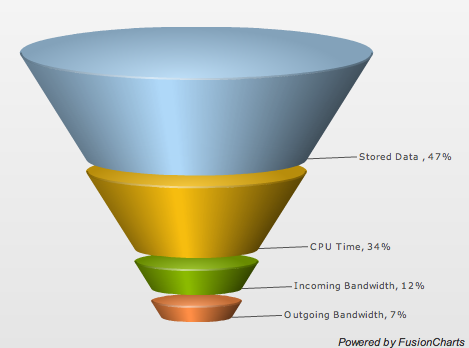
\includegraphics[scale=0.45]{img/price_div.png}}
    \subfigure[\textbf{With mailing service}.]{\label{fig:gae_cost_with_mail}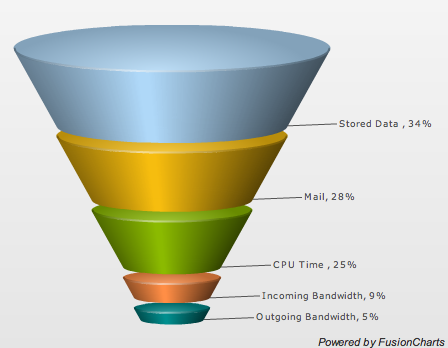
\includegraphics[scale=0.45]{img/price_div_mail.png}}
  \end{center}
  \caption{Simulated monthly cost division of resources expected to be used by one million of SmartNotes users on Google App Engine.}
  \label{fig:gae_cost}
\end{figure}


\section{Mercurial on Google App Engine}\label{sec:hg_on_gae}
\section{Cocoa user interface}\label{sec:cocoa} % System evalualtion
\chapter{System Evaluation}\label{chap:eval}
\section{Final result presentation}\label{sec:result} 
\section{Performance tests}\label{sec:performance}  % Conclusion
     
		       %% Honors theses are required to 
                          %% have an unnumbered chapter
                          %% for conclusions.  The file
                          %% Conclusion.tex should begin
                          %%   
                          %% \chapter*{Conclusion}
                          %% followed by the appropriate
                          %% text.
\begin{spacing}{1.0}
	\bibliographystyle{plain}
	\bibliography{mbib}
\end{spacing}

%\include{biblio}            %% Calls biblio.tex.  See below.
%-->\Appendix                 %% Use this command if you have one 
                          %% appendix. Use \Appendices if you 
                          %% have more than one.
	
%-->\include{toolong}         %% Calls toolong.tex which contains
                          %% an appendix.

\end{document}